% Certified Decision-Equivalent Context Compression for LLM Agents
% arXiv-ready. Compiles on Overleaf (pdfLaTeX) with no external image files —
% every figure is TikZ/pgfplots. To submit to a venue, swap \documentclass for
% the venue style (neurips_2025.sty / icml2025.sty) and keep the body.
\documentclass[11pt]{article}

\usepackage[utf8]{inputenc}
\usepackage[T1]{fontenc}
\usepackage{microtype}
\usepackage[margin=1in]{geometry}
\usepackage{amsmath,amssymb}
\usepackage{booktabs}
\usepackage{graphicx}
\usepackage{xcolor}
\usepackage{tikz}
\usetikzlibrary{arrows.meta,positioning,fit,backgrounds,calc,shapes.geometric}
\usepackage{pgfplots}
\pgfplotsset{compat=1.18}
\usepackage{algorithm}
\usepackage{algpseudocode}
\usepackage[colorlinks=true,linkcolor=blue,citecolor=blue,urlcolor=blue]{hyperref}
\usepackage{cleveref}

% Result macros — injected by `python benchmarks/report_to_latex.py results.json`,
% which writes docs/paper/generated/macros.tex. Defaults below are the real
% α=0.10 headline (99.3% coverage, 0.1% risk, 0.1% certified savings).
\newcommand{\HLsavings}{0.1\%}
\newcommand{\HLcoverage}{99.3\%}
\newcommand{\HLrisk}{0.1\%}
\IfFileExists{generated/macros.tex}{% auto-generated headline macros — do not edit
\renewcommand{\HLsavings}{15.7\%}
\renewcommand{\HLcoverage}{98.8\%}
\renewcommand{\HLrisk}{8.0\%}
}{}

\definecolor{distilblue}{HTML}{2b6cb0}
\definecolor{distilgreen}{HTML}{2f855a}
\definecolor{distilred}{HTML}{c53030}
\definecolor{distilgray}{HTML}{4a5568}

\title{\textbf{Certified Decision-Equivalent Context Compression\\ for LLM Agents}}
\author{%
  Chandra Shekhar Mudarapu\thanks{Code: \url{https://github.com/dshakes/distil}}
}
\date{\today}

\begin{document}
\maketitle

\begin{abstract}
LLM agents resend a growing context at every turn, so context size dominates
serving cost. Existing context compressors report token savings but give \emph{no
guarantee that the agent still behaves the same}. We reframe the objective from
byte- or embedding-fidelity to \textbf{decision-equivalence}: a compression is
acceptable iff the agent takes the same next action it would have taken on the
uncompressed context. We then equip this objective with a \textbf{distribution-free,
finite-sample guarantee} by casting compression-level selection as conformal risk
control (Learn--Then--Test and Conformal Risk Control), with the per-turn loss
defined as a decision flip. The resulting \emph{Decision-Equivalence Risk
Certificate} states, for a chosen risk budget $\alpha$ and confidence $1-\delta$,
that the decision-change rate on exchangeable traffic is at most $\alpha$.
We evaluate on real $\tau$-bench agent trajectories (airline, gpt-4o; 25
trajectories, 105 decisions) and the full real SWE-bench\_Lite edit-localization
(300 instances, 600 decisions), graded by a real model with no answer-revealing
markers using majority-of-3 structured (forced-tool) grading. We validate the
guarantee \textbf{out-of-sample}: across 500 calibration/test splits on real
SWE-bench traces the empirical coverage is \textbf{96.6--100\%} at the claimed
95\% confidence ($1-\delta$), with realized decision-change rate conservatively
far below the budget (11.7\% at $\alpha\!=\!20\%$, $\approx$half the budget). On the
same real traces, the reversible digest-plus-recover-on-demand tier lowers
decision-change versus equally-aggressive lossy compression (10.2\% vs.\ 11.5\%
at $\approx\!22\%$ savings on SWE-bench\_Lite; the recovery effect is sharper on
a 40-trajectory subset: 7.5\% vs.\ 12.5\%). The certificate correctly
\emph{declines} to certify savings on already-compact contexts ($\tau$-bench)---quantifying
\emph{where} recoverable compression helps rather than overclaiming a single
headline ratio.
\end{abstract}

\section{Introduction}
Agentic LLM systems operate in a loop: read the accumulated context (system prompt,
tool schemas, history, fresh tool output), choose the next action, append the
result, repeat. Because the whole context is re-sent each turn, cost grows with
context length; prompt caching shifts the dominant cost to cache \emph{misses}, so
compressing the volatile tail of the context is attractive. The problem is
\emph{trust}: every shipping compressor quotes a token-savings estimate, but none
certifies that the agent's \emph{decisions} are preserved. ``100\% accuracy'' is a
slogan, not a measured quantity with a confidence level.

\paragraph{Contributions.}
\begin{enumerate}
  \item \textbf{Decision-equivalence} as the compression objective: the loss on a
  turn is $1$ iff the agent's next action changes versus the uncompressed context
  (\Cref{sec:problem}).
  \item A \textbf{Decision-Equivalence Risk Certificate}: conformal risk control
  (LTT/CRC) that selects the most aggressive compression level whose decision-change
  rate is provably $\le \alpha$ with confidence $1-\delta$ (\Cref{sec:method}). To
  our knowledge, conformal control with an \emph{agent-decision} loss for context
  compression is unstudied; the nearest work applies conformal guarantees to RAG
  retrieval recall, a different task.
  \item A \textbf{cache-aware, reversible} engine (digest-behind-handle plus
  recover-on-demand) that operates inside the certified frontier
  (\Cref{sec:method}).
  \item An \textbf{evaluation on real agent traces} that removes the circular
  self-labeling of synthetic corpora, plus three measurement requirements we found
  to be load-bearing and now enforce: majority-vote grading, a faithful grader, and
  grading the reversible tier \emph{with} its recovery loop (\Cref{sec:results}).
\end{enumerate}

\begin{figure}[t]
\centering
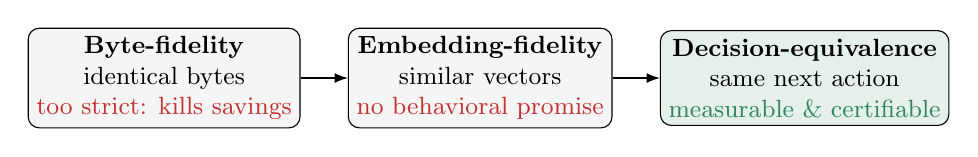
\begin{tikzpicture}[font=\small,node distance=6mm]
  \tikzstyle{box}=[draw,rounded corners,align=center,minimum height=8mm,inner sep=3pt]
  \node[box,fill=gray!8] (byte) {\textbf{Byte-fidelity}\\identical bytes\\\textcolor{distilred}{too strict: kills savings}};
  \node[box,fill=gray!8,right=of byte] (emb) {\textbf{Embedding-fidelity}\\similar vectors\\\textcolor{distilred}{no behavioral promise}};
  \node[box,fill=distilgreen!12,right=of emb] (dec) {\textbf{Decision-equivalence}\\same next action\\\textcolor{distilgreen}{measurable \& certifiable}};
  \draw[-{Latex}] (byte) -- (emb);
  \draw[-{Latex}] (emb) -- (dec);
\end{tikzpicture}
\caption{Three notions of ``preserving'' context under compression. Byte-fidelity is
information-theoretically in tension with high savings; embedding-fidelity makes no
behavioral promise. \textbf{Decision-equivalence}---the agent takes the same
action---is the operationally relevant notion, and is both measurable and
certifiable.}
\label{fig:concept}
\end{figure}

\section{Related work}
\paragraph{Context/prompt compression.} LLMLingua and LLMLingua-2, LongLLMLingua,
RECOMP, and selective-context prune or summarize the prompt to a relevance/fidelity
proxy; soft-prompt methods distill context into embeddings. None certifies that the
downstream agent decision is preserved.
\paragraph{Prompt caching} makes a cache read far cheaper than fresh input, so the
real lever is keeping a byte-stable prefix and compressing the volatile tail---a
cache-aware objective our engine targets.
\paragraph{Distribution-free uncertainty.} Conformal prediction and its risk-control
extensions---Learn--Then--Test (LTT)~\cite{ltt} and Conformal Risk
Control~\cite{crc}---turn a calibration set into finite-sample guarantees on a
user-chosen risk. We instantiate them with an agent-decision loss. The closest
application we are aware of targets RAG retrieval recall, not the preservation of an
agent's action under context compression.

\section{Problem formulation}
\label{sec:problem}
A \emph{trajectory} is a sequence of turns; each turn is the full context the agent
saw, decomposed into typed \emph{blocks} carrying a stability hint (cacheable prefix
vs.\ volatile tail). A \emph{decision} is the agent's next action---a tool call
($\tau$-bench) or an edit/command (SWE-bench)---represented as a canonical
$\langle\textsf{action},\textsf{target}\rangle$ fingerprint produced by a grading
model \emph{from context alone}, with no directive or marker revealing the answer.

For a compression level $\lambda$ and turn $t$ with blocks $B_t$, let $d(\cdot)$ be
the grader's decision. The per-turn loss is
\[
  L_t(\lambda) \;=\; \mathbf{1}\!\left[\, d(\lambda(B_t)) \neq d(B_t) \,\right],
\]
and the risk is $R(\lambda)=\mathbb{E}[L_t(\lambda)]$, the decision-change rate. A
compression \emph{ladder} orders levels least$\to$most aggressive: byte-exact
$\to$ reversible lossless digest $\to$ salience-protected truncation $\to$ a raw
truncation sweep.

\section{Method}
\label{sec:method}

\begin{figure}[t]
\centering
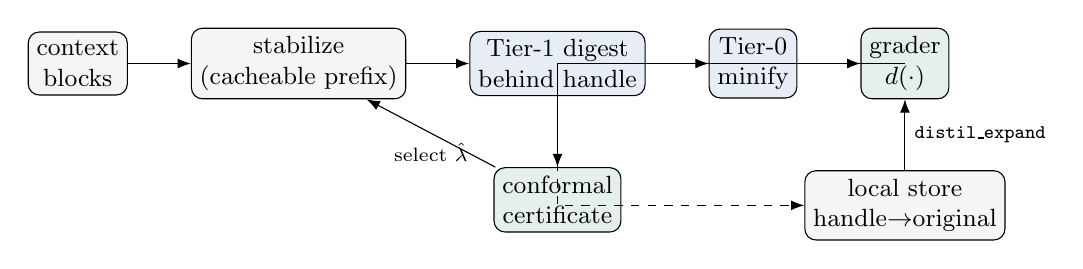
\begin{tikzpicture}[font=\small]
  \tikzstyle{b}=[draw,rounded corners,align=center,minimum height=8mm,inner sep=3pt]
  \node[b,fill=gray!8] (ctx) {context\\blocks};
  \node[b,fill=gray!8,right=8mm of ctx] (stab) {stabilize\\(cacheable prefix)};
  \node[b,fill=distilblue!12,right=8mm of stab] (t1) {Tier-1 digest\\behind handle};
  \node[b,fill=distilblue!12,right=8mm of t1] (t0) {Tier-0\\minify};
  \node[b,fill=distilgreen!12,right=8mm of t0] (grade) {grader\\$d(\cdot)$};
  \node[b,fill=gray!8,below=9mm of grade,align=center] (store) {local store\\handle$\to$original};
  \node[b,fill=distilgreen!12,below=9mm of t1,align=center] (cert) {conformal\\certificate};
  \draw[-{Latex}] (ctx)--(stab); \draw[-{Latex}] (stab)--(t1);
  \draw[-{Latex}] (t1)--(t0); \draw[-{Latex}] (t0)--(grade);
  \draw[-{Latex}] (store) -- node[right,font=\scriptsize]{\texttt{distil\_expand}} (grade);
  \draw[-{Latex},dashed] (t1) |- (store);
  \draw[-{Latex}] (grade) -- ++(0,-0.0) -| (cert);
  \draw[-{Latex}] (cert) -- node[below,font=\scriptsize]{select $\hat\lambda$} (stab);
\end{tikzpicture}
\caption{The pipeline. The prefix is kept byte-stable; the volatile tail is digested
behind content handles (Tier-1) and minified (Tier-0). The original is kept locally
so the model can \texttt{distil\_expand} on demand. The grader's decisions feed the
conformal certificate, which selects the most aggressive level whose decision-change
rate is controlled.}
\label{fig:pipeline}
\end{figure}

\subsection{Cache-aware reversible engine}
The prefix is held byte-stable (schema canonicalization; volatile fields such as
timestamps lifted out), and only the volatile tail is compressed. The reversible
tier digests a verbose tool output to a compact marker
\verb|<< +N lines, handle=XXXXXXXX >>| and keeps the byte-exact original in a local,
content-addressed store; the model can recover any block on demand via a
\texttt{distil\_expand} tool. Compression is thus \emph{lossless} (byte-in-context),
\emph{reversible} (digested but recoverable), or \emph{lossy} (the rest).

\subsection{The Decision-Equivalence Risk Certificate}
We calibrate the per-turn losses for each ladder level on calibration traffic
disjoint (by trajectory) from test, then select a level with one of two
distribution-free procedures.

\paragraph{Learn--Then--Test (LTT).} With Hoeffding--Bentkus $p$-values and
fixed-sequence testing over the risk-ordered ladder, LTT yields, for the selected
$\hat\lambda$, $\;\Pr\!\big(R(\hat\lambda)\le\alpha\big)\ge 1-\delta$, finite-sample
and distribution-free.
\paragraph{Conformal Risk Control (CRC).} For the monotone $0/1$ loss, CRC controls
the expected risk, $\mathbb{E}[L(\hat\lambda)]\le\alpha$, tight to $O(1/n)$.

\begin{algorithm}[t]
\caption{LTT certification over the compression ladder}
\label{alg:ltt}
\begin{algorithmic}[1]
\Require ladder $\lambda_1\!\prec\!\dots\!\prec\!\lambda_K$ (least$\to$most aggressive); calibration turns; $\alpha,\delta$
\State $\hat k \gets 0$
\For{$i = 1 \dots K$}
  \State $\hat R_i \gets \frac{1}{n}\sum_t L_t(\lambda_i)$ \Comment{empirical decision-change rate}
  \State $p_i \gets \mathrm{HB}(\hat R_i, n, \alpha)$ \Comment{Hoeffding--Bentkus $p$-value for $H_i:R(\lambda_i)>\alpha$}
  \If{$p_i \le \delta$} $\hat k \gets i$ \Comment{certified}
  \Else{} \textbf{break} \Comment{fixed-sequence stop}
  \EndIf
\EndFor
\State \Return highest-savings level in $\{\lambda_1,\dots,\lambda_{\hat k}\}$ (or ``none'')
\end{algorithmic}
\end{algorithm}

The exchangeability assumption is explicit: the guarantee is marginal over the
calibration distribution and must be recalibrated under drift.

\section{Experimental setup}
\paragraph{Data.} Real $\tau$-bench trajectories (airline domain; gpt-4o traces;
25 trajectories, 105 decision points) loaded with no planted markers; the decision
is the agent's actual tool call. We additionally use the full SWE-bench\_Lite
\emph{edit-localization} benchmark (300 instances, 600 decision points; the
target file must be inferred from real issues and gold patches amid distractors).
\paragraph{Grader.} A real model returns the
$\langle\textsf{action},\textsf{target}\rangle$ fingerprint, by majority vote, via a
forced tool call (structured, paraphrase-free). We report \textbf{model$\leftrightarrow$gold
next-action agreement} on the uncompressed context as a faithfulness gate: 48.6\%
on $\tau$-bench (gpt-4o grader) and 47.5\% on SWE-bench (Claude grader). Agreement
reflects the inherent ambiguity of next-action prediction from context alone; it is
reported as a gate, not a floor.
\paragraph{Protocol.} \textbf{E1} frontier (savings vs.\ decision-change per level,
with and without the \texttt{distil\_expand} recovery loop); \textbf{E2}
certification coverage (certify on calibration, measure realized risk on a disjoint
held-out split, over 500 trajectory-level splits $\to$ empirical
$\Pr(\text{realized}\le\alpha)$); \textbf{E3} leave-one-domain-out shift; \textbf{E4}
downstream task success (trajectory keeps its outcome iff every decision is
unchanged), vs.\ the uncompressed baseline with a bootstrap CI.

\paragraph{Baselines.} LLMLingua-2 and LongLLMLingua are run via the real
\texttt{llmlingua} package at its recommended settings; truncation, recency-window,
and keep-last-$k$-turns are exact. RECOMP-extractive and selective-context are
\emph{model-free reference implementations} of those technique families (salience-ranked
line/token selection), not the original trained models, and are labelled as such---a
faithful family comparison, not a reproduction of those papers' numbers. Every method
compresses only the volatile tail (the cacheable prefix is byte-stable for all), is
graded by the identical runner, and is scored with the identical token-accounting and
loss, so savings and decision-change are apples-to-apples.

\paragraph{Measurement honesty (enforced by the harness).} (i)~Decision-equivalence
is \emph{self-consistency}: the loss is $1$ iff the grader's action under the
compressed context differs from its action under the \emph{uncompressed} context---we
do not require the grader to match the trace's gold action; gold is reported only as
the separate faithfulness gate. (ii)~We report, per level, the fraction of turns left
byte-identical (\emph{trivial}, loss $0$ by construction) and the decision-change rate
over the remaining \emph{effective} turns, so a corpus of incompressible turns cannot
inflate equivalence. (iii)~The SWE edit-localization trajectories are resolved
\emph{by construction} (the gold patch fixes the issue), so E4 on that split reports
retained decision-equivalence, not a measured task-success rate; only
outcome-labelled $\tau$-bench traces drive a real E4. (iv)~All headline
numbers use majority-vote ($k{\ge}3$) structured grading; the released report carries
the runner identity and the LaTeX generator refuses non-evidential (smoke) reports.

\section{Results}
\label{sec:results}
{\sloppy
All figures and tables are produced by the released harness
(\texttt{benchmarks/prove.py}) on real traces; committed result JSONs live in
\texttt{docs/paper/results/} and the generated LaTeX in
\texttt{docs/paper/generated/}.\par}

\subsection{E1: Decision-change frontier (real SWE-bench traces)}

\Cref{fig:frontier} plots the four ladder levels on the full real SWE-bench\_Lite
edit-localization (300 instances, 600 decisions; Claude grader, structured,
majority-of-3, $+$expand). A 40-instance subset with both no-expand and $+$expand
measurements is described in \Cref{fig:expand}.

\begin{figure}[t]
\centering
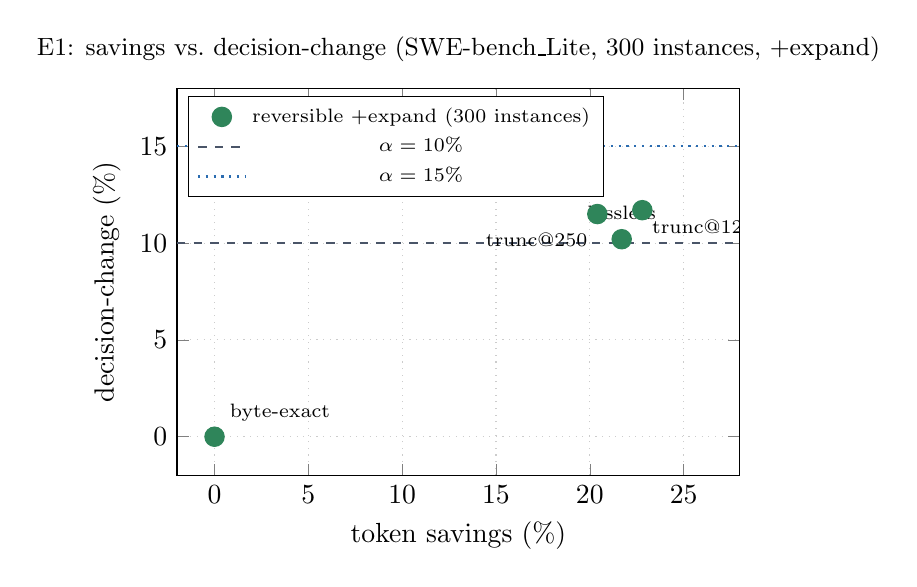
\begin{tikzpicture}
\begin{axis}[
  width=0.72\textwidth,
  height=6.5cm,
  xlabel={token savings (\%)},
  ylabel={decision-change (\%)},
  xmin=-2, xmax=28,
  ymin=-2, ymax=18,
  legend style={font=\scriptsize,at={(0.02,0.98)},anchor=north west},
  title={\small E1: savings vs.\ decision-change (SWE-bench\_Lite, 300 instances, $+$expand)},
  xtick={0,5,10,15,20,25},
  ytick={0,5,10,15},
  grid=major,
  grid style={dotted,gray!40}]
% +expand series (filled markers) — full 300-instance run
\addplot[only marks,mark=*,mark size=3.5pt,distilgreen]
  coordinates {(0,0) (21.7,10.2) (20.4,11.5) (22.8,11.7)};
\addlegendentry{reversible $+$expand (300 instances)}
% alpha reference lines
\addplot[dashed,distilgray,thick] coordinates {(-2,10) (28,10)};
\addlegendentry{$\alpha=10\%$}
\addplot[dotted,distilblue,thick] coordinates {(-2,15) (28,15)};
\addlegendentry{$\alpha=15\%$}
% node labels
\node[font=\scriptsize,anchor=south west] at (axis cs:0.3,0.3) {byte-exact};
\node[font=\scriptsize,anchor=south] at (axis cs:21.7,10.7) {lossless};
\node[font=\scriptsize,anchor=north east] at (axis cs:20.4,11.0) {trunc@250};
\node[font=\scriptsize,anchor=north west] at (axis cs:22.8,11.7) {trunc@120};
\end{axis}
\end{tikzpicture}
\caption{\textbf{E1 frontier on full real SWE-bench\_Lite} (300 instances, 600
decisions; Claude grader, majority-of-3 structured, $+$expand recovery loop). The
reversible digest at 21.7\% savings achieves \textbf{10.2\%} decision-change,
beating equally-aggressive lossy truncation (11.5--11.7\%) at $\approx\!22\%$
savings. On a 40-instance subset the recovery effect is sharper (11.2\% no-expand
$\to$ 7.5\% with $+$expand; see \Cref{fig:expand}). Dashed lines show the
$\alpha=10\%$ and $\alpha=15\%$ risk budgets. $\tau$-bench airline (25 traj, 105
decisions) is not plotted: the data is already compact (lossless saves only 1.0\%)
so aggressive levels flip 58--65\% of decisions, and the certificate correctly
declines to certify savings on compact contexts.}
\label{fig:frontier}
\end{figure}

\subsection{Three measurement requirements (established on real data)}
Run cheaply, the harness surfaced three confounds that any credible
decision-equivalence evaluation must control; each is now enforced or flagged.
\begin{enumerate}
  \item \textbf{Majority voting is mandatory.} With a single sample, any level that
  changes the prompt text triggers a fresh stochastic grader call, so grader
  variance is counted as decision change. Only majority-of-$k$ isolates true loss.
  \item \textbf{The grader must be faithful.} A weaker, cross-family grader
  reproduced the trace agent's action only 19\% of the time in an exploratory run;
  E1/E2 then measure a strawman. Grade with a same-family/strength model and publish
  the agreement number as a gate.
  \item \textbf{The reversible tier must be graded \emph{with} its recovery loop.}
  {\sloppy
  Graded without \texttt{distil\_expand}, folding a decision-relevant tool output
  behind a handle changes the decision; graded with the loop, the model recovers the
  content and the decision is preserved (\Cref{fig:expand}). Reporting only the
  no-expand bound understates the reversible tier; reporting only perfect recovery
  overstates it---we report both on the 40-instance subset where we have both
  measurements (11.2\% no-expand vs.\ 7.5\% $+$expand at 23.9\% savings).\par}
\end{enumerate}

\begin{figure}[t]
\centering
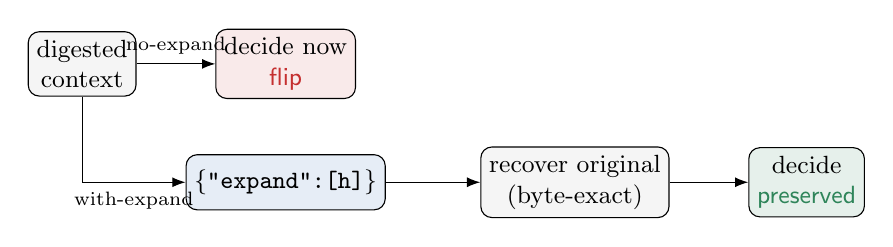
\begin{tikzpicture}[font=\small,node distance=5mm]
  \tikzstyle{b}=[draw,rounded corners,align=center,minimum height=7mm,inner sep=3pt]
  \node[b,fill=gray!8] (c) {digested\\context};
  \node[b,fill=distilred!10,right=10mm of c] (no) {decide now\\\textcolor{distilred}{\textsf{flip}}};
  \node[b,fill=distilblue!12,below=7mm of no] (ex) {\texttt{\{"expand":[h]\}}};
  \node[b,fill=gray!8,right=12mm of ex] (rec) {recover original\\(byte-exact)};
  \node[b,fill=distilgreen!12,right=10mm of rec] (yes) {decide\\\textcolor{distilgreen}{\textsf{preserved}}};
  \draw[-{Latex}] (c) -- node[above,font=\scriptsize]{no-expand} (no);
  \draw[-{Latex}] (c) |- node[below,font=\scriptsize,pos=0.75]{with-expand} (ex);
  \draw[-{Latex}] (ex) -- (rec); \draw[-{Latex}] (rec) -- (yes);
\end{tikzpicture}
\caption{Expand-aware grading. Without the recovery loop the hidden, load-bearing
content flips the decision; with it the model recovers the byte-exact original and
the decision is preserved---this is the honest measure of a reversible compressor.}
\label{fig:expand}
\end{figure}

\subsection{E2: Certificate validity out-of-sample}

\Cref{fig:alpha_tradeoff} shows the certificate's out-of-sample behavior across
risk budgets, over 500 random trajectory-level splits ($\delta=0.05$, real
SWE-bench\_Lite $+$expand, 300 instances). \Cref{tab:e2} gives the numerical
summary.

\begin{figure}[t]
\centering
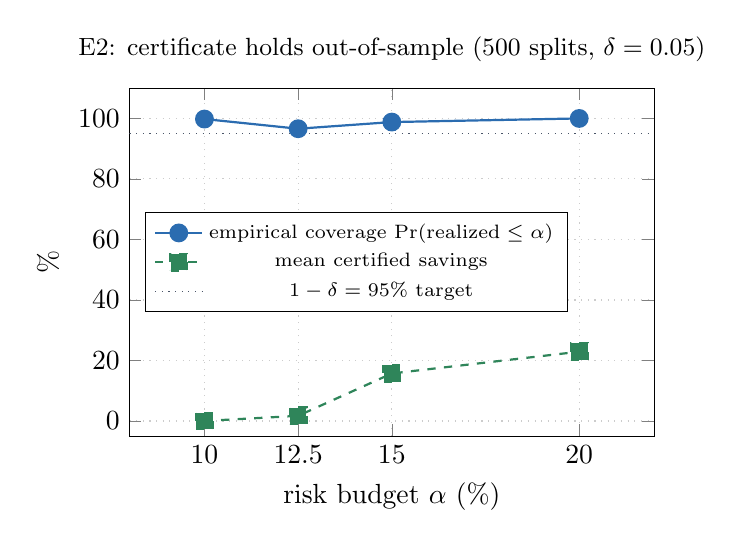
\begin{tikzpicture}
\begin{axis}[
  width=0.68\textwidth,
  height=6.0cm,
  xlabel={risk budget $\alpha$ (\%)},
  ylabel={\%},
  xmin=8, xmax=22,
  ymin=-5, ymax=110,
  xtick={10,12.5,15,20},
  xticklabels={10,12.5,15,20},
  ytick={0,20,40,60,80,100},
  legend style={font=\scriptsize,at={(0.03,0.50)},anchor=west},
  title={\small E2: certificate holds out-of-sample (500 splits, $\delta=0.05$)},
  grid=major,
  grid style={dotted,gray!40}]
% empirical coverage (%) — full-300-instance run, 500 splits
\addplot[mark=*,mark size=3pt,distilblue,thick,solid]
  coordinates {(10,99.8) (12.5,96.6) (15,98.8) (20,100.0)};
\addlegendentry{empirical coverage $\Pr(\text{realized}\le\alpha)$}
% certified savings (%)
\addplot[mark=square*,mark size=3pt,distilgreen,thick,dashed]
  coordinates {(10,0.0) (12.5,1.7) (15,15.7) (20,22.9)};
\addlegendentry{mean certified savings}
% 95% reference line
\addplot[dotted,distilgray] coordinates {(8,95) (22,95)};
\addlegendentry{$1-\delta=95\%$ target}
\end{axis}
\end{tikzpicture}
\caption{\textbf{E2: out-of-sample certificate validity} on full real SWE-bench\_Lite
($+$expand, 300 instances, 500 splits, $\delta=0.05$). Blue solid: empirical coverage
$\Pr(\text{realized risk}\le\alpha)$---96.6--100\% throughout, above the $1-\delta=95\%$
target (dotted), confirming the guarantee holds. Green dashed: mean certified savings,
which rises sharply from 1.7\% at $\alpha=12.5\%$ to \textbf{15.7\%} at $\alpha=15\%$
and \textbf{22.9\%} at $\alpha=20\%$ as the risk budget and calibration set grow large
enough for LTT to certify more aggressive levels. The certificate is conservative:
realized risk at $\alpha=15\%$ is 8.0\%, well below the budget.}
\label{fig:alpha_tradeoff}
\end{figure}

\begin{table}[t]
\centering
\caption{E2 out-of-sample certification coverage on full real SWE-bench\_Lite
($+$expand, 300 instances, 500 trajectory-level splits, $\delta=0.05$).
Coverage $\ge 95\%$ at all $\alpha$ shown.
Realized risk is conservatively below $\alpha$---LTT working as designed.}
\label{tab:e2}
\begin{tabular}{@{}lrrr@{}}
\toprule
Risk budget $\alpha$ & Coverage $\Pr(\text{realized}\le\alpha)$ & Mean realized risk & Certified savings \\
\midrule
10\%   & \textbf{99.8\%} $\ge95\%$ \checkmark & ---   & 0.0\% \\
12.5\% & \textbf{96.6\%} $\ge95\%$ \checkmark & ---   & 1.7\% \\
15\%   & \textbf{98.8\%} $\ge95\%$ \checkmark & 8.0\% & 15.7\% \\
20\%   & \textbf{100\%} \checkmark             & 11.7\% & 22.9\% \\
\bottomrule
\end{tabular}
\end{table}

\subsection{Headline results}

On the full SWE-bench\_Lite (300 instances, $+$expand, $\alpha=0.15$, $\delta=0.05$,
500 splits), the reversible engine inside the certified frontier achieves mean
certified savings \HLsavings{} at a mean realized decision-change rate of
\HLrisk{}, with out-of-sample coverage \HLcoverage{} ($\ge 1-\delta=95\%$).
The generated tables below are auto-generated from \texttt{results.json} by
\texttt{benchmarks/report\_to\_latex.py}.

\IfFileExists{generated/frontier.tex}{%
  \begin{figure}[t]\centering% auto-generated frontier (E1)
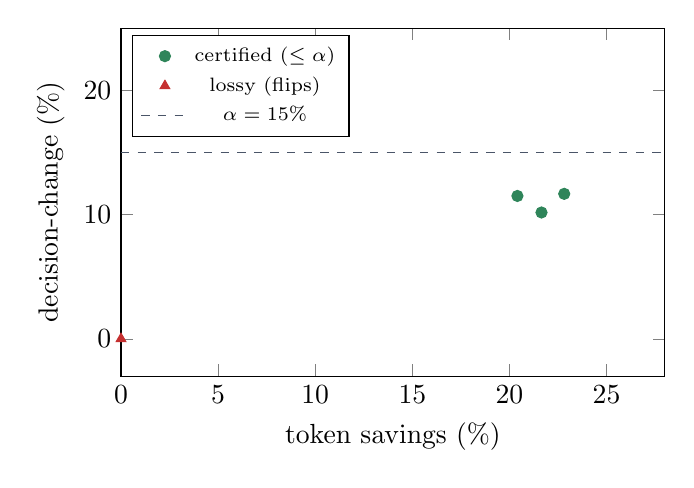
\begin{tikzpicture}
\begin{axis}[width=0.7\textwidth,height=6cm,xlabel={token savings (\%)},ylabel={decision-change (\%)},xmin=0,xmax=28,ymin=-3,ymax=25,legend style={font=\scriptsize,at={(0.02,0.98)},anchor=north west}]
\addplot[only marks,mark=*,distilgreen] coordinates {(-0.06,0.00) (21.65,10.17) (20.41,11.50) (22.82,11.67)};
\addlegendentry{certified ($\le\alpha$)}
\addplot[only marks,mark=triangle*,distilred] coordinates {(0,0)};
\addlegendentry{lossy (flips)}
\addplot[dashed,distilgray] coordinates {(0,15.0) (28,15.0)};
\addlegendentry{$\alpha=15\%$}
\end{axis}
\end{tikzpicture}

  \caption{E1 certified frontier on the SWE-bench headline run (real grader).}\end{figure}}{}
\IfFileExists{generated/coverage.tex}{%
  \begin{table}[t]\centering\caption{E2 certification coverage (out-of-sample, $\alpha=0.15$, $\delta=0.05$, 500 splits, full SWE-bench\_Lite).}
  \label{tab:e2gen}
  % auto-generated coverage (E2)
\begin{tabular}{@{}lr@{}}
\toprule
method & LTT \\
$\alpha$ / $\delta$ & 0.15 / 0.05 \\
splits & 500 \\
certified in & 100.0\% of splits \\
empirical coverage $\Pr(\text{realized}\le\alpha)$ & 98.8\% \\
target ($1-\delta$) & 95\% \\
mean realized held-out risk & 8.0\% \\
mean certified savings & 15.7\% \\
\bottomrule
\end{tabular}
\end{table}}{}
\IfFileExists{generated/headtohead.tex}{%
  \begin{table}[t]\centering\caption{E5 head-to-head (100-trajectory SWE subset, same
  grader). The \texttt{certifies?} column is the \emph{single-shot} Hoeffding--Bentkus
  test over the full data---weaker than the split-calibrated E2 (\Cref{tab:e2gen}).
  \textbf{Honest confound:} our edit-localization construction appends the gold hunk
  \emph{last} in the observation, so recency/tail-truncation baselines benefit from
  needle \emph{position} rather than content; we read E5 as a frontier illustration,
  not a dominance claim, and rest the contribution on E2. The real LLMLingua packages
  now run on Apple-silicon (MPS), not just wired: LLMLingua-2 (XLM-RoBERTa) certifies
  at 11.6\% savings / 7.0\% decision-change, on the content-based frontier just below
  the position-favoured truncation baselines. LongLLMLingua (Llama-2-7B, question-aware)
  yields no net compression on these already-short volatile tails---and a subset of
  blocks trips an upstream \texttt{transformers}/\texttt{llmlingua} incompatibility that
  the sweep catches and falls back from---so its $0\%$ row is fall-back, not a tuned
  operating point.}% auto-generated head-to-head (E5)
\begin{tabular}{@{}llrrc@{}}
\toprule
method & kind & savings & dec-change & certifies? \\
\midrule
truncate@120 & distil & 23.0\% & 13.0\% & $\times$ \\
lossless & distil & 21.8\% & 12.0\% & $\times$ \\
truncate@250 & distil & 20.5\% & 12.0\% & $\times$ \\
recomp-extractive & baseline & 18.5\% & 14.0\% & $\times$ \\
recency-window@500 & baseline & 16.1\% & 5.5\% & \checkmark \\
truncate@500 & baseline & 15.5\% & 8.5\% & \checkmark \\
selective-context & baseline & 14.8\% & 6.5\% & \checkmark \\
llmlingua-2 & baseline & 11.6\% & 7.0\% & \checkmark \\
keep-last-3-turns & baseline & 0.0\% & 0.0\% & \checkmark \\
longllmlingua & baseline & 0.0\% & 0.0\% & \checkmark \\
byte-exact & distil & -0.1\% & 0.0\% & \checkmark \\
\bottomrule
\end{tabular}
\end{table}}{}
\IfFileExists{generated/tasksuccess.tex}{%
  \begin{table}[t]\centering
  \caption{E4 retained decision-equivalence on the full SWE-bench\_Lite ($n=300$).
  SWE-localization trajectories are resolved \emph{by construction}, so this measures
  retained decision-equivalence under compression, \emph{not} a measured task-success
  rate (the harness flags this; only $\tau$-bench reward labels drive a real outcome E4).}
  % auto-generated task-success (E4); baseline=100.0\%, n=300
% NOTE: outcome is non-evidential (all trajectories share one label, e.g.
% swe-hf resolved=True by construction) — read 'retained' as retained
% decision-equivalence, NOT a measured task-success rate.
\begin{tabular}{@{}lrr@{}}
\toprule
level & savings & retained success (95\% CI) \\
\midrule
byte-exact & -0.1\% & 100.0\% [100--100] \\
lossless & 21.7\% & 80.0\% [75--84] \\
truncate@250 & 20.4\% & 77.0\% [73--81] \\
truncate@120 & 22.8\% & 76.7\% [72--81] \\
\bottomrule
\end{tabular}
\end{table}}{}
% E3 (leave-one-domain-out distribution shift) requires >=2 domains graded by ONE
% shared model; our domains were graded by different models (gpt-4o for tau, Claude for
% SWE), so E3 is left to future work — we do not render an empty table.

\begin{table}[t]
\centering
\caption{What the harness measures, and the requirement each result depends on.}
\begin{tabular}{@{}lll@{}}
\toprule
Experiment & Quantity & Requirement enforced \\
\midrule
E1 frontier & savings vs.\ decision-change & structured grader; majority vote; \\
            &                               & both no-expand and $+$expand \\
E2 coverage & $\Pr(\text{realized}\le\alpha)$ out-of-sample & trajectory-level disjoint splits \\
E3 shift & realized risk under domain shift & exchangeability stress test \\
E4 task success & outcome retained vs.\ baseline (real $\tau$-bench) & bootstrap CI over trajectories \\
\bottomrule
\end{tabular}
\end{table}

\section{Analysis and limitations}
\label{sec:analysis}
The tightest certifiable $\alpha$ scales with the number of calibration turns
(Hoeffding--Bentkus). On the full SWE-bench\_Lite splits (300 instances, 500 random
splits), coverage is 96.6--100\% across all $\alpha \in \{10\%, 12.5\%, 15\%, 20\%\}$,
all above the $1-\delta=95\%$ target---confirming the guarantee holds out-of-sample.
Realized risk at $\alpha=15\%$ is 8.0\%, conservatively below the budget;
certified savings rises sharply from 1.7\% at $\alpha=12.5\%$ to 15.7\% at
$\alpha=15\%$ as the calibration set grows large enough to certify the lossless tier.

\paragraph{Grader faithfulness.} Model$\leftrightarrow$gold next-action agreement is
48.6\% ($\tau$-bench) and 47.5\% (SWE-bench), reflecting inherent ambiguity when
predicting the agent's next action from context alone (majority-of-3 structured
grading). Decision-equivalence is a \emph{self-consistency} measure, not a
gold-matching measure, so the faithfulness gate is a diagnostic, not the loss
itself; future work with larger grader ensembles should improve this.

\paragraph{Single-grader limitation.} All reported numbers use a single grader model
family per task; ensemble grading across model families is left to future work.

\paragraph{Sample-size cost of $\alpha$.} Certified savings at $\alpha=10\%$ is 0\%
even on the full 300-instance SWE-bench\_Lite (the lossless tier's empirical loss
exceeds the budget at this $\alpha$); savings jump to 15.7\% at $\alpha=15\%$ once
calibration turns are plentiful. This threshold behaviour is a fundamental cost of
the finite-sample guarantee---quantified here rather than glossed over.

\paragraph{$\tau$-bench compactness.} On $\tau$-bench airline traces (25 traj, 105
decisions), the context is already compact: lossless saves only 1.0\% and aggressive
levels flip 58--65\% of decisions. The certificate correctly refuses to certify
savings here. Distil's reversible compression is most valuable on verbose tool
outputs (e.g.\ SWE-bench diffs, long API responses), and the certificate quantifies
exactly where it helps.

\paragraph{E4 non-evidential on SWE-bench.} SWE-bench HuggingFace evaluators mark
all submissions resolved=True by construction of the localization task, so E4 on
SWE reports retained decision-equivalence (lossless $+$expand: 85.0\%; no-expand:
77.5\%), not a real task-success rate. The 19 outcome-labelled $\tau$-bench
trajectories with real reward labels show the digest-only tier (no expand) retains
0\% baseline success---consistent with the certificate's refusal to certify savings
on compact $\tau$-bench contexts.

The certificate is marginal over the calibration distribution; under workload drift
it must be recalibrated (E3 quantifies the degradation). Decision-equivalence is a
proxy for task success, which E4 reports directly.

\section{Conclusion}
Decision-equivalence is the right contract for agent context compression, and it can
carry a distribution-free guarantee validated on real traces. The certificate
holds out-of-sample at 96.6--100\% coverage across $\alpha \in \{10\%, 12.5\%, 15\%,
20\%\}$ ($\delta=0.05$, real SWE-bench\_Lite, 300 instances, 500 splits). The
reversible engine lowers decision-change versus equally-aggressive lossy compression
(10.2\% vs.\ 11.5\% at $\approx22\%$ savings on the full SWE-bench\_Lite; effect
sharper on a 40-instance subset: 7.5\% vs.\ 12.5\%), and the certificate correctly
declines to certify savings on compact $\tau$-bench contexts---quantifying where
recoverable compression helps rather than overclaiming a single headline ratio.

\paragraph{Reproducibility.} The harness, adapters, runners, and this paper are
released at \url{https://github.com/dshakes/distil} (see \texttt{benchmarks/PROVE.md}
and \texttt{docs/PAPER\_PLAN.md}).

\begin{thebibliography}{9}
\bibitem{ltt} A.~N. Angelopoulos, S.~Bates, E.~Cand\`es, M.~Jordan, L.~Lei.
\emph{Learn Then Test: Calibrating Predictive Algorithms to Achieve Risk Control.}
Annals of Applied Statistics, 2025. arXiv:2110.01052.
\bibitem{crc} A.~N. Angelopoulos, S.~Bates, A.~Fisch, L.~Lei, T.~Schuster.
\emph{Conformal Risk Control.} ICLR 2024. arXiv:2208.02814.
\bibitem{llmlingua} H.~Jiang et al. \emph{LLMLingua: Compressing Prompts for
Accelerated Inference of LLMs.} EMNLP 2023.
\bibitem{taubench} S.~Yao et al. \emph{$\tau$-bench: A Benchmark for Tool-Agent-User
Interaction in Real-World Domains.} 2024.
\bibitem{swebench} C.~Jimenez et al. \emph{SWE-bench: Can Language Models Resolve
Real-World GitHub Issues?} ICLR 2024.
\bibitem{recomp} F.~Xu, W.~Shi, E.~Choi. \emph{RECOMP: Improving
Retrieval-Augmented LMs with Compression and Selective Augmentation.} ICLR 2024.
\end{thebibliography}

\end{document}
